\section{Neural Networks}
\label{sec:neural_networks}
Neural Networks are a learning representation which the goal is to approximate some function \( f^* \). Data collected from an environment encodes an underlying function \( \mathrm{\mathbf{y}} = f^*(\mathrm{\mathbf{x}}) \) that maps an input \( \textbf{x} \) to an output \( \mathrm{\mathbf{y}} \), which may be a category from a classifier or a continue value in regression problems. The neural network defines an approximate mapping \( \mathrm{\mathbf{y}} = f(\mathrm{\mathbf{x}};\boldsymbol{\theta}) \), by learning the values of the parameters \(\boldsymbol{\theta}\), which result in the best function approximation. Figure \ref{fig:ann} shows a neural network and an artificial neuron in detail.

\begin{figure}[!htbp]
\centering
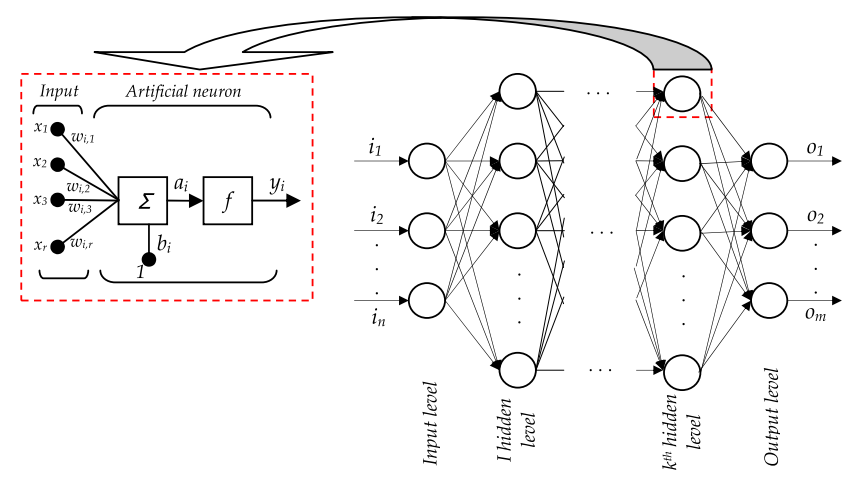
\includegraphics[width=0.8\textwidth]{Cap3/ann}
\caption{An artificial neuron within a feed forward artificial neural network \cite{dejan12}. }
\label{fig:ann}
\end{figure}

These networks are typically represented by composing together many different functions, which are associated with a directed acyclic graph, by describing a computational model. For example, we might have three layers (each of them representing a function \( f^{(1)}, f^{(2)} \), and \(f^{(3)} \)), connecting in a chain and resulting in a final representation \( f(\mathrm{\mathbf{x}}) = f^{(3)}(  f^{(2)} ( f^{(1)}(\mathrm{\mathbf{x}}))) \).

During a neural network training, the objective is to adjust \(f(\mathrm{\mathbf{x}})\) to match \(f^{*}(\mathrm{\mathbf{x}})\), by using the training dataset, which provides noisy examples of \(f^{*}(\mathrm{\mathbf{x}})\) evaluated in different points. The training examples directly specify what the output layer must do at each point \(\mathrm{\mathbf{x}}\), but the learning algorithm must decide how to use all layers to produce this desired output \cite{Goodfellow-et-al-2016}.

Additionally, we must also choose a learning algorithm to tune this function approximation. In the context of neural networks, gradient-based algorithms are broadly used, especially those based on the backpropagation idea \cite{hinton88}. The purpose of these algorithms are to propagate the gradient of a cost function through the whole network, in order to minimize the cost function. Most modern neural networks perform this optimization strategy, by using maximum likelihood, i.e. the cross-entropy between the training data and the model distribution:

\begin{equation}
J(\boldsymbol{\theta}) = -\mathbb{E}_{\mathrm{\mathbf{x}},\mathrm{\mathbf{y}}\sim \hat{p}_{data}}\log{p_{model}(\mathrm{\mathbf{y}} | \mathrm{\mathbf{x}})}
\label{eq:cost_function_ml}
\end{equation}

In this work, we used the mean squared error loss function, in order to fit the dataset. Indeed, we may show that both cost functions are closely related. Let us consider normally distributed errors:

\begin{equation}
{p_{model}(\bvec{y} | \bvec{x})} = \mathcal{N}( \bvec{y}; f (\bvec{x}; \boldsymbol{\theta}), \sigma^{2}\bvec{I})
\label{eq:errors}
\end{equation}
where \(f (\bvec{x}; \boldsymbol{\theta})\) and \(\sigma^{2}\bvec{I}\)  are the mean and covariance of this distribution. By substituting Eq. \eqref{eq:errors} in Eq. \eqref{eq:cost_function_ml}:

\begin{equation}
J(\boldsymbol{\theta}) = \frac{1}{2}\mathbb{E}_{\bvec{x},\bvec{y}\sim \hat{p}_{data}} \lVert \bvec{y} - f (\bvec{x}; \boldsymbol{\theta}) \rVert ^{2} + const
\label{eq:cost_function_expectation}
\end{equation} 

The constant term does not depend on \( \boldsymbol{\theta} \) and may be dropped. By explicitly evaluating the expectation in Eq. \eqref{eq:cost_function_expectation}, we arrive at the mean squared error cost function:

\begin{equation}
J(\boldsymbol{\theta}) = \frac{1}{2m} \sum^{m}_{i} \lVert y_{i} - f (\bvec{x}; \boldsymbol{\theta}) \rVert ^{2}
\end{equation}

Lastly, the gradient of the loss function is taken and propagated through the hidden layers by the chain rule. For example, given \(\textbf{Y} = g(\textbf{X}) \) and \(z = f(\textbf{Y}) \), then the chain rule states:

\begin{equation}
\nabla_{\textbf{X}}z = \sum_{j}(\nabla_\textbf{X}Y_{j})  \frac{\partial{z}}{\partial{Y_{j}}}
\end{equation}

This equation is recursively taken, until the gradient is propagated to all layers of the neural network.
